% ─────────────────────────────────────────────────────────────────────────────
%  pm4-github-insights — System Architecture Diagram
%  Compile with: pdflatex system-architecture.tex
% ─────────────────────────────────────────────────────────────────────────────
\documentclass[border=18pt]{standalone}
\usepackage{tikz}
\usepackage{xcolor}
\usetikzlibrary{arrows.meta, positioning, fit, backgrounds, calc}

% ── Colour palette (Material Design 200/300) ─────────────────────────────────
\definecolor{cExt}{HTML}{C5CAE9}   % indigo-200    — External
\definecolor{cIng}{HTML}{81D4FA}   % light-blue-300 — Ingestion
\definecolor{cBrk}{HTML}{FFCC80}   % orange-300    — Broker
\definecolor{cPrc}{HTML}{A5D6A7}   % green-300     — Processing
\definecolor{cSto}{HTML}{CE93D8}   % purple-300    — Storage
\definecolor{cApi}{HTML}{FFF176}   % yellow-300    — API
\definecolor{cViz}{HTML}{F48FB1}   % pink-300      — Visualization
\definecolor{cDock}{HTML}{ECEFF1}  % blue-grey-50  — Docker outer

% ── Node / group / arrow styles ───────────────────────────────────────────────
\tikzset{
  svc/.style 2 args={
    draw=#1!70!black, fill=#1!35, thick,
    rounded corners=6pt,
    minimum width=3.6cm, minimum height=1.8cm,
    text width=3.4cm, align=center,
    inner sep=7pt,
    font=\small\sffamily
  },
  grpborder/.style={
    draw=#1!60!black, fill=#1!12,
    thick, dashed, rounded corners=10pt, inner sep=14pt
  },
  arr/.style={-{Stealth[length=5pt,width=3pt]}, thick, #1},
  darr/.style={-{Stealth[length=4pt,width=3pt]}, thick, dashed, gray!70},
  lbl/.style={
    font=\tiny\sffamily,
    fill=white, fill opacity=0.9, text opacity=1,
    inner sep=1pt, rounded corners=2pt
  },
}

\begin{document}
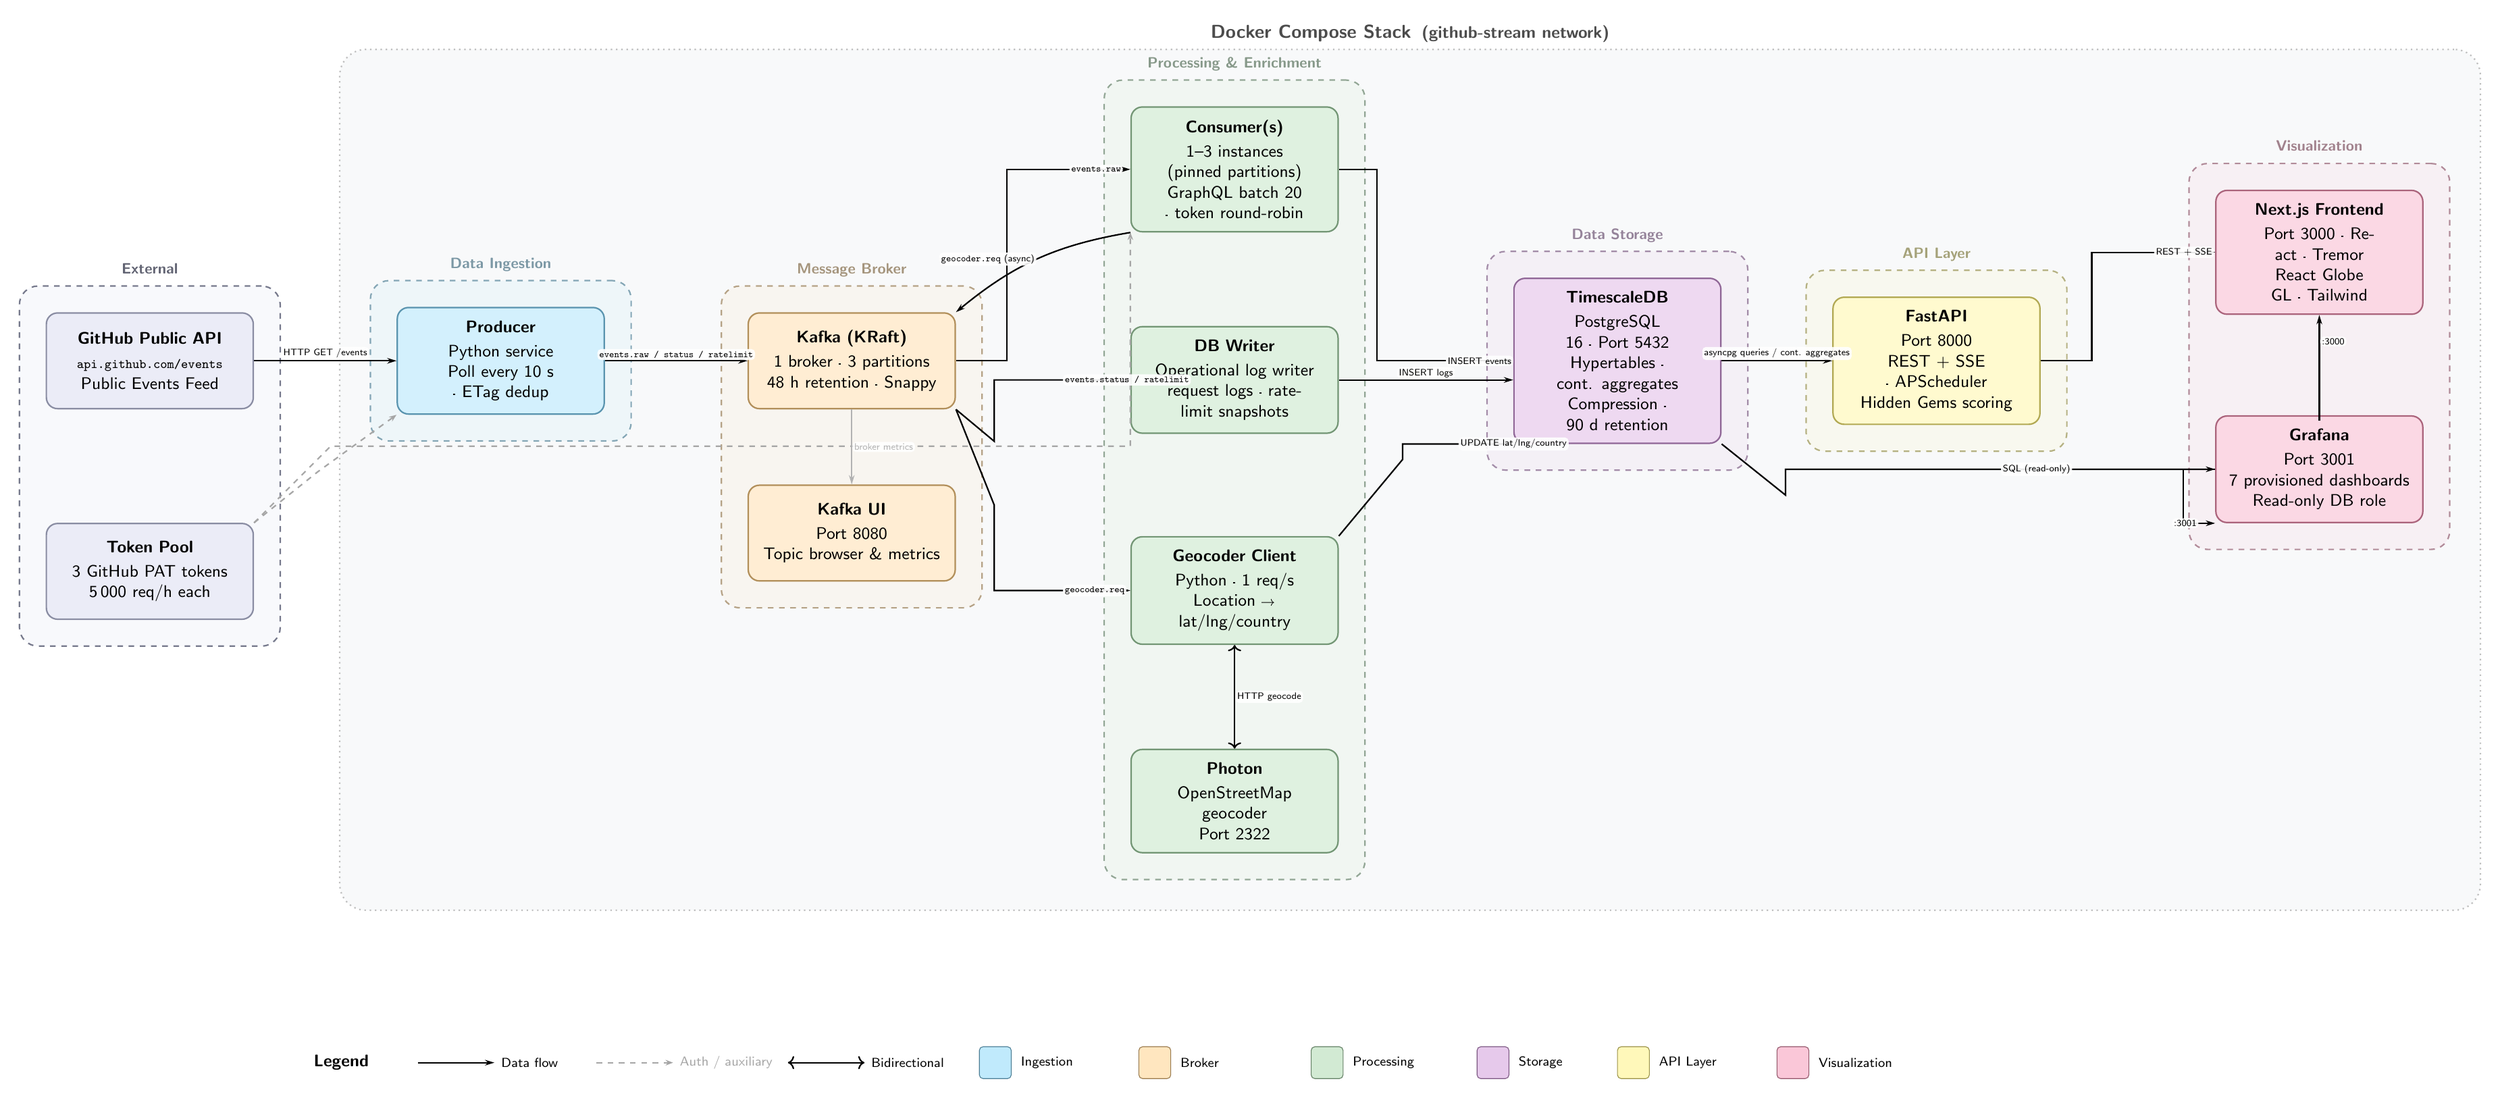
\begin{tikzpicture}[x=1.2cm, y=1.2cm]

% ═══════════════════════════════════════════════════════════════════════════════
%  NODES
% ═══════════════════════════════════════════════════════════════════════════════

% ── External (col 0) ──────────────────────────────────────────────────────────
\node[svc={cExt}{}] (github)  at ( 0,  2.5) {
  \textbf{GitHub Public API}\\[2pt]
  {\fontsize{7}{9}\texttt{api.github.com/events}}\\
  {\fontsize{7}{9} Public Events Feed}
};
\node[svc={cExt}{}] (tokens)  at ( 0, -0.8) {
  \textbf{Token Pool}\\[2pt]
  {\fontsize{7}{9} 3 GitHub PAT tokens}\\
  {\fontsize{7}{9} 5\,000 req/h each}
};
\node[svc={cExt}{}] (user)    at (34,  0.8) {
  \textbf{End User}\\[2pt]
  {\fontsize{7}{9} Browser}
};

% ── Ingestion — col 1 ─────────────────────────────────────────────────────────
\node[svc={cIng}{}] (producer) at ( 5.5,  2.5) {
  \textbf{Producer}\\[2pt]
  {\fontsize{7}{9} Python service}\\
  {\fontsize{7}{9} Poll every 10 s · ETag dedup}
};

% ── Broker — col 2 ────────────────────────────────────────────────────────────
\node[svc={cBrk}{}] (kafka)   at (11,  2.5) {
  \textbf{Kafka (KRaft)}\\[2pt]
  {\fontsize{7}{9} 1 broker · 3 partitions}\\
  {\fontsize{7}{9} 48 h retention · Snappy}
};
\node[svc={cBrk}{}] (kafkaui) at (11, -0.2) {
  \textbf{Kafka UI}\\[2pt]
  {\fontsize{7}{9} Port 8080}\\
  {\fontsize{7}{9} Topic browser \& metrics}
};

% ── Processing — col 3 ────────────────────────────────────────────────────────
\node[svc={cPrc}{}] (consumer)  at (17,  5.5) {
  \textbf{Consumer(s)}\\[2pt]
  {\fontsize{7}{9} 1–3 instances (pinned partitions)}\\
  {\fontsize{7}{9} GraphQL batch 20 · token round-robin}
};
\node[svc={cPrc}{}] (dbwriter)  at (17,  2.2) {
  \textbf{DB Writer}\\[2pt]
  {\fontsize{7}{9} Operational log writer}\\
  {\fontsize{7}{9} request logs · rate-limit snapshots}
};
\node[svc={cPrc}{}] (geoclient) at (17, -1.1) {
  \textbf{Geocoder Client}\\[2pt]
  {\fontsize{7}{9} Python · 1 req/s}\\
  {\fontsize{7}{9} Location → lat/lng/country}
};
\node[svc={cPrc}{}] (photon)    at (17, -4.4) {
  \textbf{Photon}\\[2pt]
  {\fontsize{7}{9} OpenStreetMap geocoder}\\
  {\fontsize{7}{9} Port 2322}
};

% ── Storage — col 4 ───────────────────────────────────────────────────────────
\node[svc={cSto}{}] (timescale) at (23,  2.5) {
  \textbf{TimescaleDB}\\[2pt]
  {\fontsize{7}{9} PostgreSQL 16 · Port 5432}\\
  {\fontsize{7}{9} Hypertables · cont. aggregates}\\
  {\fontsize{7}{9} Compression · 90 d retention}
};

% ── API Layer — col 5 ─────────────────────────────────────────────────────────
\node[svc={cApi}{}] (fastapi) at (28,  2.5) {
  \textbf{FastAPI}\\[2pt]
  {\fontsize{7}{9} Port 8000}\\
  {\fontsize{7}{9} REST + SSE · APScheduler}\\
  {\fontsize{7}{9} Hidden Gems scoring}
};

% ── Visualization — col 6 ─────────────────────────────────────────────────────
\node[svc={cViz}{}] (frontend) at (34,  4.2) {
  \textbf{Next.js Frontend}\\[2pt]
  {\fontsize{7}{9} Port 3000 · React · Tremor}\\
  {\fontsize{7}{9} React Globe GL · Tailwind}
};
\node[svc={cViz}{}] (grafana) at (34,  0.8) {
  \textbf{Grafana}\\[2pt]
  {\fontsize{7}{9} Port 3001}\\
  {\fontsize{7}{9} 7 provisioned dashboards}\\
  {\fontsize{7}{9} Read-only DB role}
};

% ═══════════════════════════════════════════════════════════════════════════════
%  GROUP BORDERS
% ═══════════════════════════════════════════════════════════════════════════════
\begin{scope}[on background layer]

  \node[grpborder={cExt},
        fit=(github)(tokens),
        label={[font=\fontsize{8}{10}\sffamily\bfseries, color=cExt!50!black, inner sep=3pt] above:\strut External}
  ] (grpExt) {};

  \node[grpborder={cIng},
        fit=(producer),
        label={[font=\fontsize{8}{10}\sffamily\bfseries, color=cIng!50!black, inner sep=3pt] above:\strut Data Ingestion}
  ] (grpIng) {};

  \node[grpborder={cBrk},
        fit=(kafka)(kafkaui),
        label={[font=\fontsize{8}{10}\sffamily\bfseries, color=cBrk!50!black, inner sep=3pt] above:\strut Message Broker}
  ] (grpBrk) {};

  \node[grpborder={cPrc},
        fit=(consumer)(dbwriter)(geoclient)(photon),
        label={[font=\fontsize{8}{10}\sffamily\bfseries, color=cPrc!50!black, inner sep=3pt] above:\strut Processing \& Enrichment}
  ] (grpPrc) {};

  \node[grpborder={cSto},
        fit=(timescale),
        label={[font=\fontsize{8}{10}\sffamily\bfseries, color=cSto!50!black, inner sep=3pt] above:\strut Data Storage}
  ] (grpSto) {};

  \node[grpborder={cApi},
        fit=(fastapi),
        label={[font=\fontsize{8}{10}\sffamily\bfseries, color=cApi!50!black, inner sep=3pt] above:\strut API Layer}
  ] (grpApi) {};

  \node[grpborder={cViz},
        fit=(frontend)(grafana),
        label={[font=\fontsize{8}{10}\sffamily\bfseries, color=cViz!50!black, inner sep=3pt] above:\strut Visualization}
  ] (grpViz) {};

  \node[draw=gray!50, thick, dotted, fill=cDock, fill opacity=0.35,
        rounded corners=14pt, inner sep=16pt,
        fit=(grpIng)(grpBrk)(grpPrc)(grpSto)(grpApi)(grpViz),
        label={[font=\normalsize\sffamily\bfseries, color=gray!60!black]
               above:\textbf{Docker Compose Stack}\enspace{\small(github-stream network)}}
  ] (docker) {};

\end{scope}

% ═══════════════════════════════════════════════════════════════════════════════
%  ARROWS
% ═══════════════════════════════════════════════════════════════════════════════

% GitHub API → Producer
\draw[arr={}]
  (github.east) -- node[lbl, above] {HTTP GET /events}
  (producer.west);

% Token Pool → Producer (events auth)
\draw[darr]
  (tokens.north east) -- ++(1.0, 0.8) -- (producer.south west);

% Token Pool → Consumer (GraphQL auth)
\draw[darr]
  (tokens.north east) -- ++(1.2, 1.2) -| (consumer.south west);

% Producer → Kafka
\draw[arr={}]
  (producer.east) -- node[lbl, above] {\texttt{events.raw / status / ratelimit}}
  (kafka.west);

% Kafka → Kafka UI (monitoring)
\draw[arr={gray!60}]
  (kafka.south) -- node[lbl, right] {broker metrics}
  (kafkaui.north);

% Kafka → Consumer
\draw[arr={}]
  (kafka.east) -- ++(0.8, 0) |- node[lbl, near end, right] {\texttt{events.raw}}
  (consumer.west);

% Kafka → DB Writer
\draw[arr={}]
  (kafka.south east) -- ++(0.6, -0.5) |- node[lbl, near end, right]
    {\texttt{events.status / ratelimit}}
  (dbwriter.west);

% Kafka → Geocoder Client
\draw[arr={}]
  (kafka.south east) -- ++(0.6, -1.5) |- node[lbl, near end, right]
    {\texttt{geocoder.req}}
  (geoclient.west);

% Consumer → Kafka (geocoder loopback)
\draw[arr={}, bend right=15]
  (consumer.south west) to
    node[lbl, left] {\texttt{geocoder.req} (async)}
  (kafka.north east);

% Consumer → TimescaleDB
\draw[arr={}]
  (consumer.east) -- ++(0.6, 0) |- node[lbl, near end, right] {INSERT events}
  (timescale.west);

% DB Writer → TimescaleDB
\draw[arr={}]
  (dbwriter.east) -- node[lbl, above] {INSERT logs}
  (timescale.west |- dbwriter.east);

% Geocoder Client ↔ Photon
\draw[arr={}, <->]
  (geoclient.south) -- node[lbl, right] {HTTP geocode}
  (photon.north);

% Geocoder Client → TimescaleDB
\draw[arr={}]
  (geoclient.north east) -- ++(1.0, 1.2) |-
    node[lbl, near end, right] {UPDATE lat/lng/country}
  (timescale.south west);

% TimescaleDB → FastAPI
\draw[arr={}]
  (timescale.east) -- node[lbl, above] {asyncpg queries / cont. aggregates}
  (fastapi.west);

% TimescaleDB → Grafana
\draw[arr={}]
  (timescale.south east) -- ++(1.0, -0.8) |-
    node[lbl, near end, right] {SQL (read-only)}
  (grafana.west);

% FastAPI → Frontend
\draw[arr={}]
  (fastapi.east) -- ++(0.8, 0) |- node[lbl, near end, right] {REST + SSE}
  (frontend.west);

% User → Frontend
\draw[arr={}]
  (user.north) -- node[lbl, near end, right] {:3000}
  (frontend.south);

% User → Grafana
\draw[arr={}]
  (user.west) -- ++(-0.5, 0) |- node[lbl, near end, left] {:3001}
  (grafana.south west);

% ═══════════════════════════════════════════════════════════════════════════════
%  LEGEND
% ═══════════════════════════════════════════════════════════════════════════════
\begin{scope}[shift={(-1,-8.5)}]
  \node[font=\small\sffamily\bfseries] at (4, 0) {Legend};
  \draw[arr={}] (5.2, 0) -- ++(1.2, 0)
    node[right, font=\fontsize{7}{9}\sffamily] {Data flow};
  \draw[darr]   (8.0, 0) -- ++(1.2, 0)
    node[right, font=\fontsize{7}{9}\sffamily] {Auth / auxiliary};
  \draw[arr={}, <->] (11.0, 0) -- ++(1.2, 0)
    node[right, font=\fontsize{7}{9}\sffamily] {Bidirectional};
  \foreach \col/\name/\xpos in {
    cIng/Ingestion/14,
    cBrk/Broker/16.5,
    cPrc/Processing/19.2,
    cSto/Storage/21.8,
    cApi/{API Layer}/24,
    cViz/Visualization/26.5
  }{
    \fill[\col!50, rounded corners=2pt] (\xpos,-0.25) rectangle ++(0.5,0.5);
    \draw[\col!60!black, rounded corners=2pt] (\xpos,-0.25) rectangle ++(0.5,0.5);
    \node[font=\fontsize{7}{9}\sffamily, right] at (\xpos+0.55, 0) {\name};
  }
\end{scope}

\end{tikzpicture}
\end{document}